\section{Paralleles Licht}

\subsection{Einleitung}
In diesem versuch sollen die Gitterkonstanten $g$ zweier Filter ermittelt werden. Dies geschieht indem man paralleles Licht durch sie hindurchscheinen lässt,
auch hier wird wie im vorherigem Versuch das Licht gebrochen und es kommt zur Aufspaltung. Über die Art der Aufspaltung kann man dann auf die Gitterkonstanten schließen. \\
Um paralleles Licht zu erzeugen wird vor eine normale Taschenlampe eine Lochblende geschaltet, diese Bündelt das Licht auf einen kleine Bereich. Als nächstes fällt
das Licht auf den Filter (siehe Abbildung 3) und wird in seine spektralen Anteile zerlegt welche auf einer weißen Platte abgebildet werden.\\
Die Größen, die für die Bestimmung der Gitterkonstante benötigt werden sind:
\begin{itemize}
	\item $d$... Abstand zwischen Filter und Platte.
	\item $x$... Abstand des blauen Anteils des Spektrums zur Mitte.
	\item $k$... Anzahl der Maxima.
\end{itemize}
\begin{center}
	\begin{minipage}{0.6\textwidth}
		\begin{figure}[H]
			\centering
			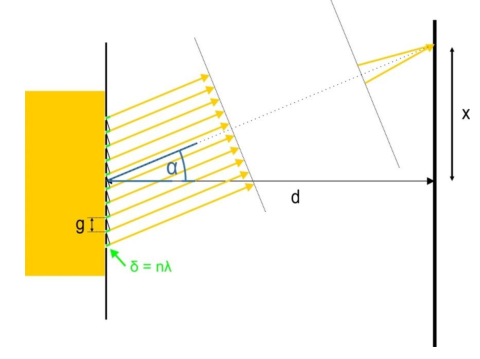
\includegraphics[scale=0.8]{C:/Users/josefk/Desktop/Spektroskopie/src/img/gitter.PNG}
			\caption{Gitter. Paralleles Licht trifft auf ein Gitter mit dem Abstand $g$ zwischen den Einzelspalten. Auf einem Schirm im
				Abstand $d$ kann eine winkelabhängige Intensitätsverteilung beobachtet werden. Ein Maximum ist erkennbar, wenn der
				Gangunterschied $\Delta s$ ein Vielfaches der Wellenlänge $\lambda$ ist.}
		\end{figure}
	\end{minipage}
\end{center}
\clearpage

\subsection{Berechnung}
\subsubsection{Gitter I (G = $500mm^{-1}$)}

Zur berechnung vod der Gitterkonstante $g$ braucht man wieder Gleichung (1) und zudem noch:
\begin{align}
	\sin \alpha = \frac{k\lambda}{a}
\end{align}
Bei Gleichung (3) wurde nur $g$ mit $a$ aus Gleichung (2) ausgetauscht. Wenn man dann Gleichung (1) und (2)\\ zusammenfügt und auf $g$ umformt, erhält man:
\begin{align*}
	g = k \lambda \frac{1}{\sin (\tan^{-1} (\frac{x}{d}))}
\end{align*}

\begin{table}[H]
	\centering
	\begin{tabular}{lcccccc}
		\toprule
		Messung & x [cm] & d [cm] & k [cm] & $\lambda$ [nm] & g[$\mu$m]   & G[mm]       \\
		\midrule
		A1      & 5      & 19,65  & 1      & 490            & 0,001987063 & 503,2552353 \\
		A2      & 5      & 19,65  & 1      & 490            & 0,001987063 & 503,2552353 \\
		A3      & 5      & 19,65  & 1      & 490            & 0,001987063 & 503,2552353 \\
		A4      & 5      & 19,65  & 1      & 490            & 0,001987063 & 503,2552353 \\
		A5      & 4,9    & 19,65  & 1      & 490            & 0,002025173 & 493,7850163 \\
		A6      & 4,9    & 19,65  & 1      & 490            & 0,002025173 & 493,7850163 \\
		\bottomrule
	\end{tabular}
	\caption{Messwerte und daraus resultierende Gitterkonstante für Gitter I}
\end{table}

\begin{itemize}
	\item Der Abstand $d$ zwischen Filter und und Platte beträgt 19.65cm.
	\item Für $\lambda$ wird eine Wellenlänge gewählt, die gut auf der Platte zu erkennen ist und dem nach sich auch leicht vermessen lässt, wir habe den übergang von grün nach blau bei 490nm gewählt.
	\item $K$ ist 1 da der Bereich in dem alle Farben zu sehen sind nur als ein Maximum zählt.
	\item $x$ wurde zur Fehlerminimierung sechs mal bestimmt.
	\item $g$ steht für die Gitterkonstante.
	\item $G$ steht für die Anzahl an Spalten, welche durch $G = \frac{1}{g}$ gegeben ist, und auf den Filtern steht.
\end{itemize}

Die berechnete Gitteranzahl beträgt 500,1 $\pm$ ...

\subsubsection{Gitter II (G = $1000mm^{-1}$)}

\begin{table}[H]
	\centering
	\begin{tabular}{lcccccc}
		\toprule
		Messung & x [cm] & d [cm] & k [cm] & $\lambda$ [nm] & g[$\mu$m]   & G[mm]       \\
		\midrule
		A1      & 4,84   & 10     & 1      & 490            & 0,001124743 & 889,091909  \\
		A2      & 4,84   & 10     & 1      & 490            & 0,001124743 & 889,091909  \\
		A3      & 4,85   & 10     & 1      & 490            & 0,001122865 & 890,5793526 \\
		A4      & 4,86   & 10     & 1      & 490            & 0,001120994 & 892,0650452 \\
		A5      & 4,85   & 10     & 1      & 490            & 0,001122865 & 890,5793526 \\
		A6      & 4,86   & 10     & 1      & 490            & 0,001120994 & 892,0650452 \\
		\bottomrule
	\end{tabular}
	\caption{Messwerte und daraus resultierende Gitterkonstante für Gitter II}
\end{table}

Die ermittelte Gitteranzahl beträgt 890,5787689 $\pm$ ...

\subsection{Diskussion}

Die Berechnete Gitterzahl vom ersten Gitter stimmt so gut wie zu 100\% mit den Herstellerangaben überein, beim 2. 
Gitter unterscheiden sich die Herstellerangaben und die und die Gemessenen um 11\%. Mögliche Fehler hierfür ist Einerseits der Umstand das $\lambda$ nicht genau ist sondern aus einer Tabelle stammt die 
in zehner Schritten steigt und andererseits die Tatsache das man den Übergang zwischen den Farben nicht klar erkennen kann. Desweiteren ist uns aufgefallen das auf einer Seite die 
Aufspaltung der Farben sehr gut zu sehen war wohingegen auf der anderen Seite diese kaum wahrgenommen werden konnten. Leider haben wir davon kein Foto.   
